\chapter{Appendix}
\section{Background to Experimental Work}
\subsection{The Kinetics of Rafting}

The thermodynamic driving force for rafting depends on the lattice misfit and applied stress.  V\'{e}ron et al. noticed that strain induced during creep seems to be responsible for the rafting phenomenon, and postulated that there is a critical density of plasticity-induced dislocations necessary to induce rafting, and that additional dislocation density above this threshold would have no influence on rafting \cite{veron96}.

A novel method was used by Matan et al.  To precisely quantify the kinetics of rafting in a commercial 2$^{nd}$ generation superalloy, CMSX 4, with the aim to evaluate the influence of rafting on creep deformation \cite{matan99}.  Interrupted creep tests at 950\celsius/185 \mega\pascal\ were performed on single crystal heat-treated creep specimens with $\left<100\right>$ orientation parallel to the applied stress, using 20 kN constant load creep testing machines.  The tests were interrupted  at 150, 280, 500, 695, 1060 and 1170 hours.  The tested specimens were sectioned axial to the direction of applied stress, and micrographs were taken and stereologically characterised.  Degree of rafting was seen to increase with the length of creep testing.

The threshold strain for rafting to proceed in the absence of applied stress was determined.  The threshold strain was found to be 0.10+/-0.03\%.  When a specimen was strained beyond the threshold strain, it continues to raft during subsequent annealing in the absence of applied stress.  If accumulated strain is below the threshold strain, subsequent annealing does not promote further raftingMatan et al.  Postulated that the thermodynamic driving force and the kinetics of rafting in the plastic regime would be correlated to the lattice misfit.  This will be investigated by looking at three alloys in the LDSX series with representative low, medium and high lattice misfits.

\subsection{Effect of Misfit on Creep Properties}

The LDSX series comprises of eight 4$^{th}$ generation alloys that has been developed at the Rolls-Royce University Technology Centre are currently undergoing evaluation.  The nominal compositions and predicted misfit values by JMatPro$^{\copyright}$ are shown in Table~\ref{tab:LDSXcomps}.

Alloys with representative low, intermediate and high misfits, LDSX--1, 6 and 8, have been chosen for this study, as seen in Figure \ref{fig:MisfitJMatPro}.  LDSX--1 is the least alloyed, with the lowest content of Mo, Re and W, and consequently, possesses the lowest misfit.  LDSX--8 has the highest refractory element content, and the highest predicted misfit.  A commerical second generation superalloy, CMSX-4, will be used as reference.
%
\begin{table}[htdp]
\begin{center}
\begin{tabular}{lccccccccccc}
\hline\hline
Alloy 	&     Ni    &  Al   &  Co  &   Cr &   Mo     &Ti     & Ta    & W     &Re &    Ru    & Hf\\
\hline
LDSX-1  &   Bal.&    6.0&    3.0&     3.0&     2.5&    0.25&    6.5&    2.9&    6.2&     3.5&     0.1\\
LDSX-2    & Bal.&    6.0&    8.0&     3.0&     5.0&    0.25&    6.5&    2.9&    6.2&     3.5&     0.1\\
LDSX-3     &Bal.&    6.0&    3.0&     3.0&     5.0&    0.25&    6.5&    4.8&    6.2&     3.5&     0.1\\
LDSX-4 &    Bal.&    6.0&    8.0&     3.0&     2.5&    0.25&    6.5&    4.8&    6.2&     3.5&     0.1\\
LDSX-5 &    Bal.&    6.0&    8.0&     3.0&     2.5&    0.25&    6.5&    2.9&    6.2&     5.0&     0.1\\
LDSX-6  &   Bal.&    6.0&    3.0&     3.0&     2.5&    0.25&    6.5&    4.8&    6.2&     5.0&     0.1\\
LDSX-7  &   Bal.&    6.0&    3.0&     3.0&     5.0&    0.25&    6.5&    2.9&    6.2&     5.0&     0.1\\
LDSX-8  &   Bal.&    6.0&    8.0&     3.0&     5.0&    0.25&    6.5&    4.8&    6.2&     5.0&     0.1\\
\hline\hline
\end{tabular}
\end{center}
\caption{Nominal compositions of LDSX--1 to 8.}\label{tab:LDSXcomps}
\end{table}
%
\begin{figure}[H]
\begin{center}
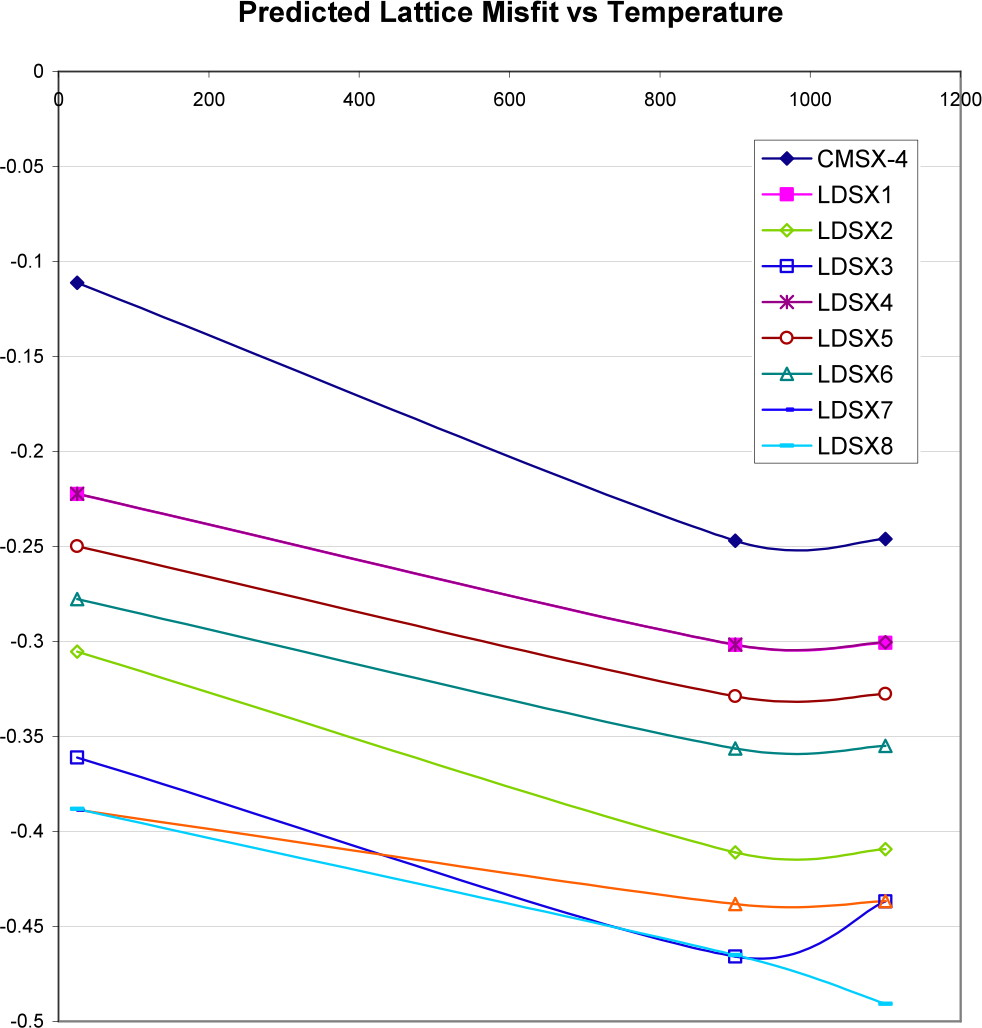
\includegraphics{MisfitJMatPro}
\caption{Predicted misfit as a function of temperature for LDSX--1, 6 and 8.}
\label{fig:MisfitJMatPro}
\end{center}
\end{figure}
%
The more heavily alloyed LDSX--6 with higher lattice misfit took a longer time than LDSX--1 to reach the same elongation.  The most heavily alloyed LDSX--8, suffered from premature rupture, and had half the rupture life of LDSX--1.  Additionally, LDSX--8 had no visible incubation period, and a mere two hours of primary creep.  This premature failure can be due to several factors.  It has a highly negative misfit, and is noted to be prone to TCP precipitation. 




\section{Experimental Work}

Bars of alloys designated LDSX--1, 6 and 8 were directionally-solidified to produce single crystals with $\left<001\right>$ orientation at the Precision Casting Facility (PCF) in Derby, England.  The bars were solution treated to eliminate casting segregation: LDSX--1 at 1340\celsius\ for 10 hours, LDSX--6 at 1340\celsius\ for 10 hours, and LDSX--8 at 1360\celsius\ for 15 hours.  They were then primary aged at 1150\celsius\ for 4 hours and secondary aged at 870\celsius\ for 16 hours to eliminate secondary $\gamma'$. 

Tensile creep specimens were machined from LDSX--1, 6 and 8.  Their $\theta$/$\rho$ angles, showing their relative orientation to the loading axis, were 4.2/36.4, 13.0/18.7 and 3.0/28.8, respectively.  They were crept at 950\celsius/375\mega\pascal\ and the tests were stopped when the onset of secondary creep was observable.  Sections were cut out from the gauge lengths of these interrupted creep specimens.  They were then subject to thermal exposure at 950\celsius, the temperature that the specimens were crept at, for a subsequent 10, 50, 100, 200, 500 or 3000 hours.  Microstructural examination was performed with a JEOL 6340F FEGSEM, where micrographs representative areas were taken to quantify microstructural stability and the extent of rafting in these alloys. 

Misfit measurements are difficult to obtain for nickel-base superalloys by diffraction using conventional laboratory X-ray sources.  The $\left<001\right>$ $\gamma$ peaks are invisible in fully ordered structures.  The $\left<001\right>$ $\gamma'$ peak is visible but it is very weak and requires a long data collection time when using a typical X-ray source available at universities.  This leads to instrumental line broadening, a source of error.  Also, the $\left<002\right>$ peaks of $\gamma$ and $\gamma'$ overlap and are very difficult to separate.  In order to split these peaks accurately, the $\left<001\right>$ $\gamma'$ peak position, which indicates its lattice parameter, can be used to ``fix" the position of the $\gamma'$ peak, which allows us to determine the peak position $\gamma$ through curve deconstruction. X-rays produced at a synchrotron are of higher intensity, and much shorter acquisition times would be required.  Measurements of the lattice parameters of the $\gamma$ matrix phases and $\gamma'$ precipitate phases of the alloys were performed on the BM28 beamline at the European Synchrotron Radiation Facility (ESRF) in Grenoble, France.  Monochromation of the X-rays was achieved by diffraction from a double-crystal Si $\{111\}$ monochromator to give an incident energy of 11.9 \kilo\electronvolt\ with a wavelength of 1.0418 \angstrom.  The beam was 0.5$\times$0.5 \milli\meter\ at full width at half maximum (FWHM), with a resolution of 1.7$\times$10$^{-4}$, and was focused on the sample surface using a torroidal mirror.

Transverse sections of the bars with $\left<001\right>$ nominally vertical were mounted on a goniometer head attached to an 11-axis Huber diffractometer.  This permitted the sample to be translated in x, y and z within the diffractometer and orientated in four circles ($\phi$ , $\chi$ , $\omega$, 2$\theta$).To establish the orientation of the sample, the 2$\theta$ angle was set at a value consistent with the expected lattice parameter of the material and $\phi$ varied until a strong diffraction signal was detected.  For samples with significant off-axis orientations, scans in $\phi$ were performed as chi was increased to locate the $\left(001\right)$ pole.  Once established, 2$\theta$ was increased to an angle consistent with diffraction from a $\left(111\right)$ pole and the sample reoriented accordingly before scanning in $\phi$ to indentify the pole.  Knowledge of the orientations of these two poles permitted automatic reorientation of the sample to other poles for detailed measurement.
%
\begin{figure}[H]
\begin{center}
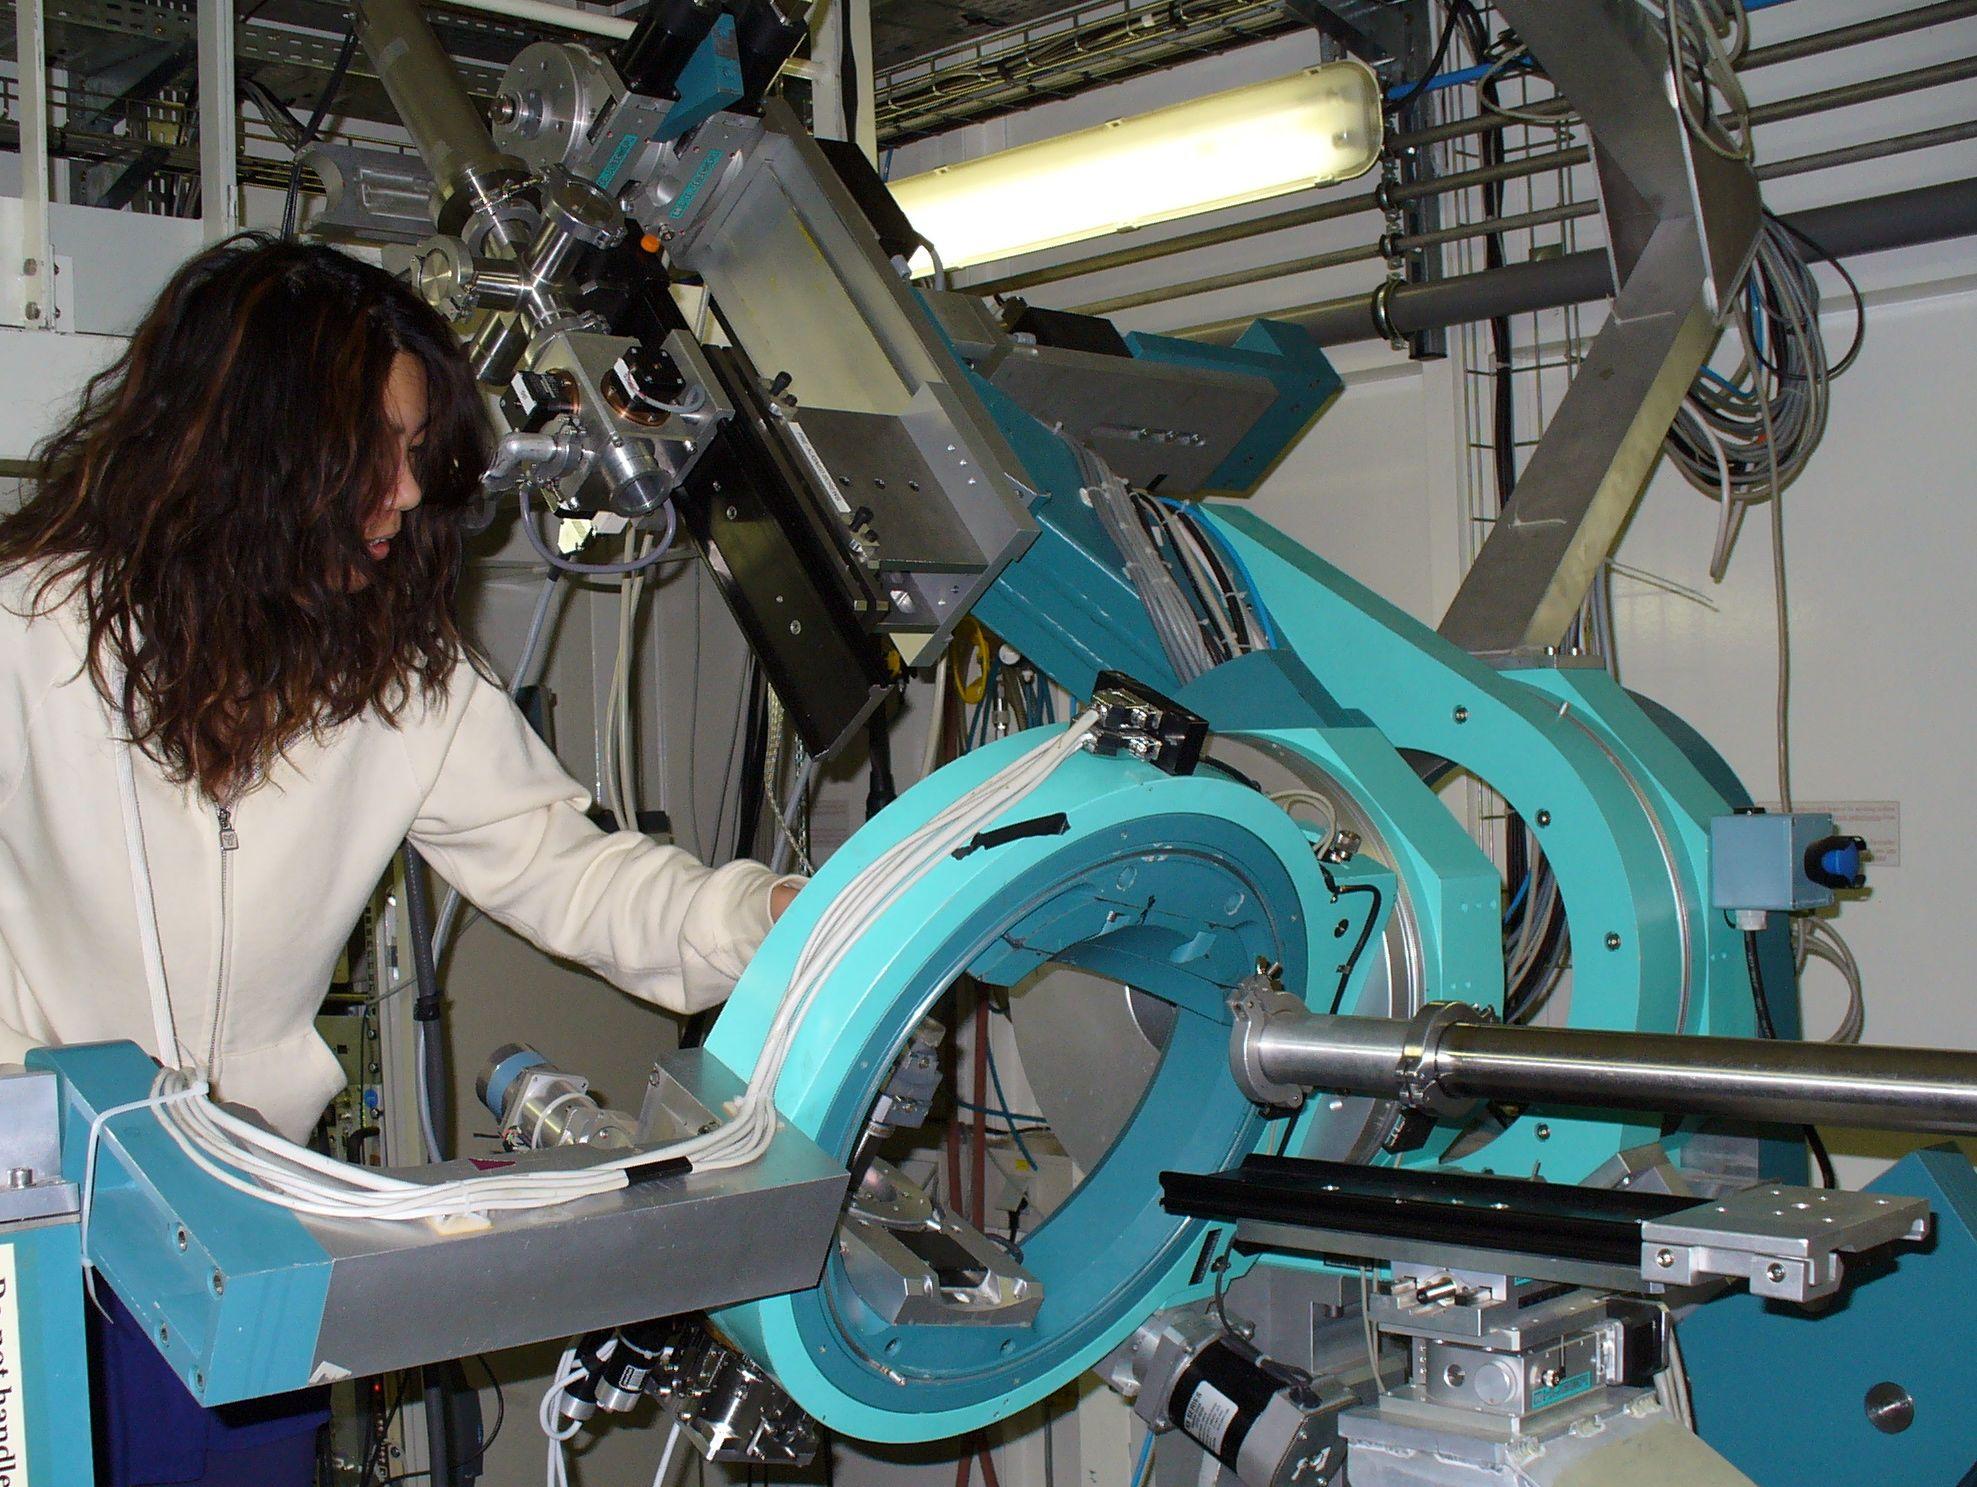
\includegraphics[width=10cm]{esrfgonio}
\caption{Placement of a diffraction sample on the goniometer attached to the 11-axis Huber diffractometer on the beamline BM28 at the European Synchrotron Facility.}\label{fig:esrfgonio}
\end{center}
\end{figure}
%
The $\left(001\right)$ \& $\left(003\right)$ superlattice reflections and $\left(002\right)$ \& $\left(004\right)$ fundamental reflections were scanned in \emph{h} \& \emph{k} to generate two-dimensional reciprocal space maps.  It was considered necessary to characterise the superlattice reflections so that the lattice parameter of the $\gamma'$ could be uniquely determined and enable unambiguous identification of the contribution of the $\gamma'$ to the overlapping fundamental reflections.  The low atomic scattering contrast between the atoms occupying the face and corner sites in the $\gamma'$ necessitated long acquisition times for the superlattice reflections.  Three dimensional reciprocal space maps showing intensity in $h$ and $k$ were generated by stepping $h$ and $k$ in increments of 0.0025 \angstrom\ at 1 second per point.  The measured misfit values were compared with values predicted by JMatPro$^{\copyright}$.The interfacial dislocation networks form during creep as a result of $\frac{a}{2}\left<110\right>\{111\}$ creep dislocations being held up at the $\gamma$/$\gamma'$ interface. Misfit can also be calculated by measuring the average dislocation spacing along the $\left<110\right>$ direction in these networks through TEM observation.

\section{Results and Discussion}

\subsection{Microstructural Stability and Degree of Rafting}

LDSX--1, 6 and 8 all display the onset of rafting prior to the presence of applied load (Figure \ref{fig:LDSXAsAged}).  When subject to interrupted creep at an intermediate temperature of 950\celsius, LDSX--1 and 6 raft perpendicular to the direction of applied stress (Figure \ref{fig:LDSXInterrupted}).  The more highly misfitting LDSX--6 rafts quicker and more extensively than LDSX--1.  On the other hand, LDSX--8, predicted by JMatPro$^{\copyright}$ to have a highly negative misfit, undergoes substantial precipitate coarsening in all 3 $\left<001\right>$ directions prior to stress being applied.  This has been termed the labyrinth structure.  This is unusual; superalloys generally raft only after sufficient plastic deformation has occurred ~\cite{reed99}.

After further thermal exposure, LDSX--1 continues rafting, with marked precipitate coalescence after 200 hours (Figure \ref{fig:LDSXInterrupted_200}).  LDSX--1 shows a stable phase structure over the timescale of these tests; TCP precipitation was unusual, even after 500 additional hours at 950\celsius (Figure \ref{fig:LDSXInterrupted_500}).  This shows that creep rupture in LDSX--1 was not due to phase instability.
%
\begin{figure}[hp]
\begin{center}
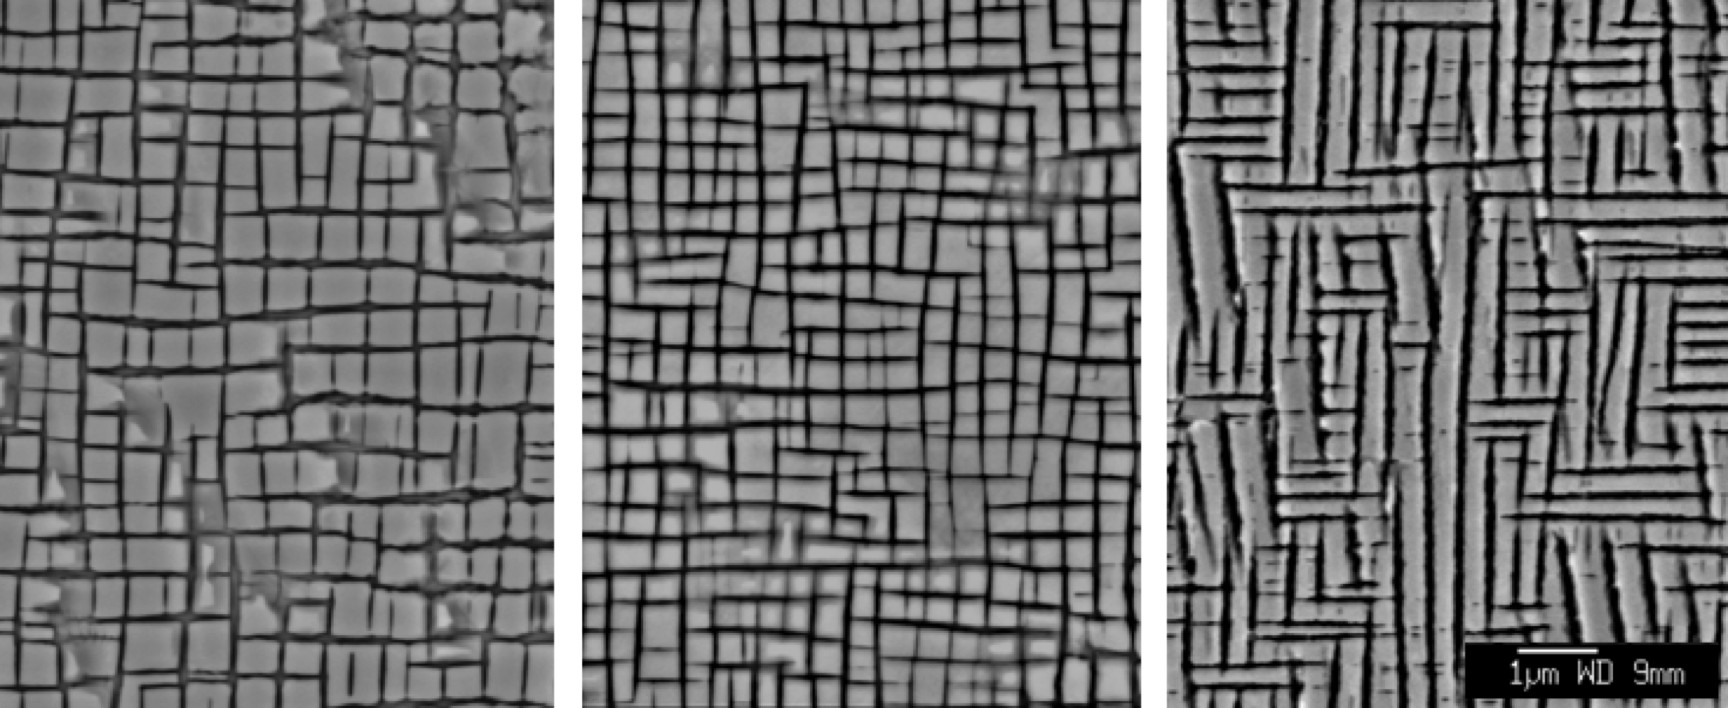
\includegraphics{LDSXAsAged}
\caption{LDSX--1, 6 and 8: as aged}\label{fig:LDSXAsAged}
\end{center}
\end{figure} 
%
\begin{figure}[hp]
\begin{center}
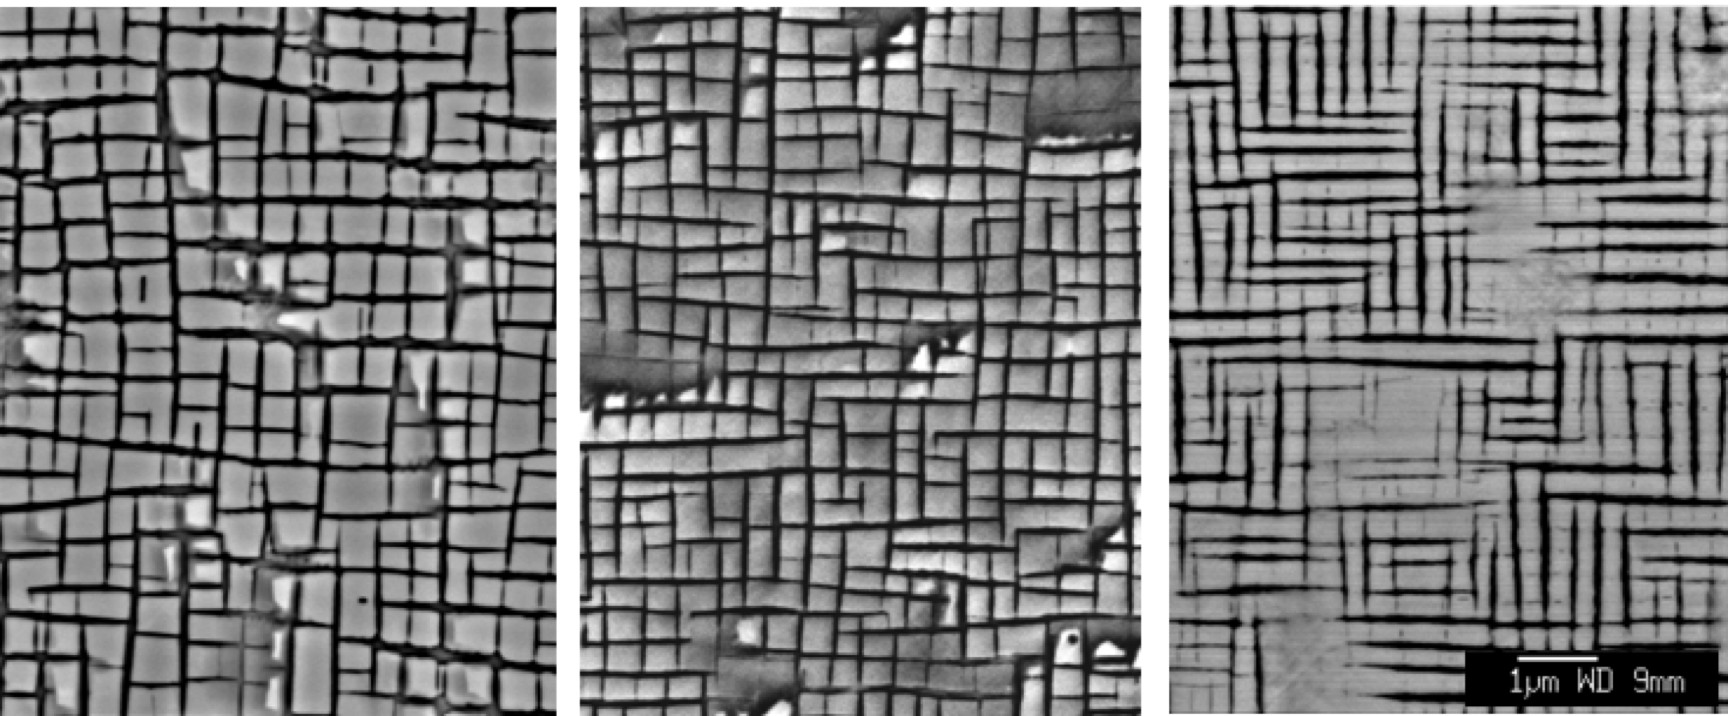
\includegraphics{LDSXInterrupted}
\caption{LDSX--1, 6 and 8: as interrupted crept }\label{fig:LDSXInterrupted}
\end{center}
\end{figure} 
%
\begin{figure}[hp]
\begin{center}
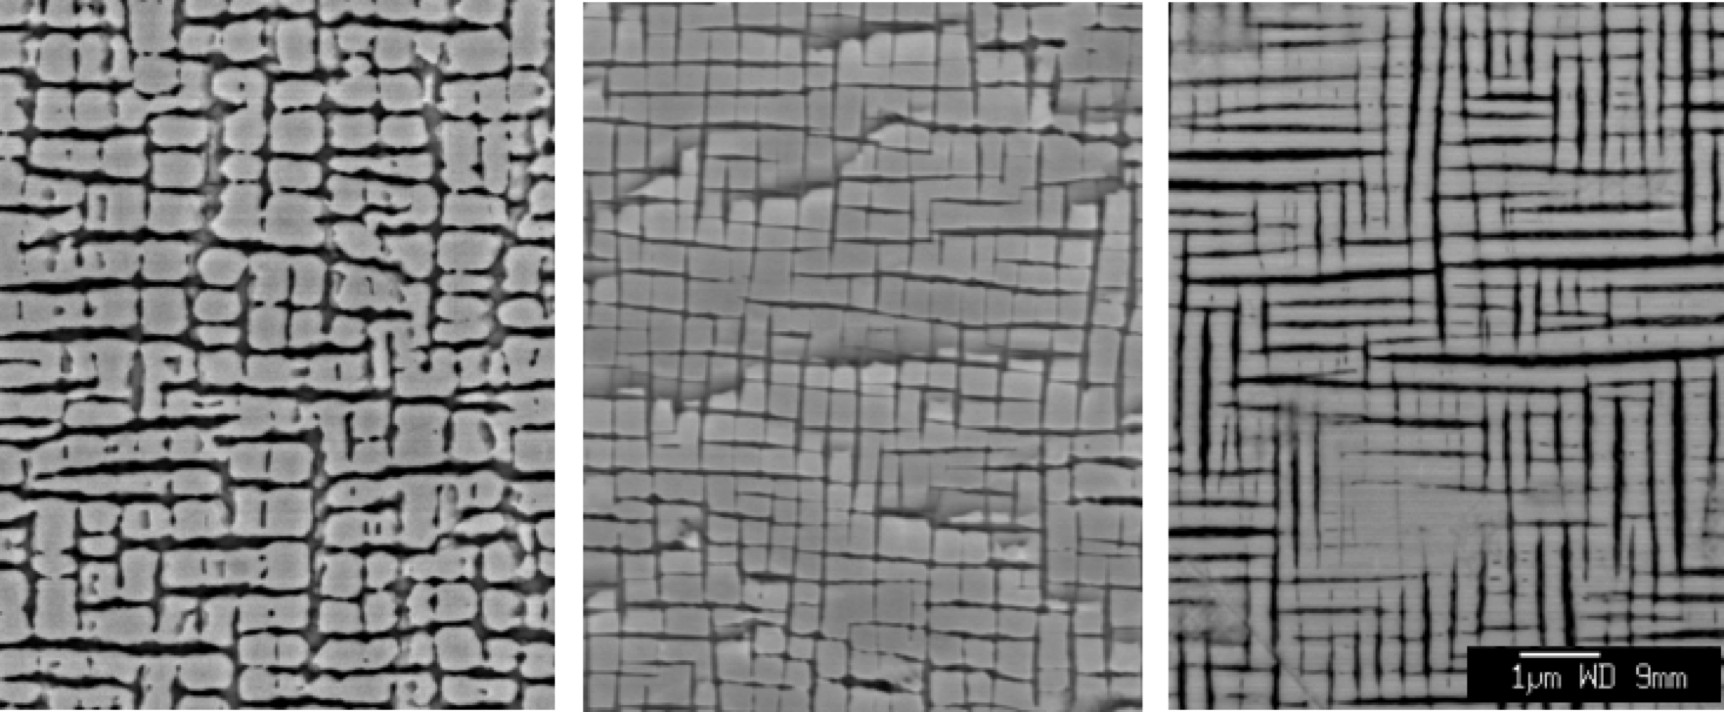
\includegraphics{LDSXInterrupted_10}
\caption{LDSX--1, 6 and 8: as interrupted crept + 10 hours at 950\celsius}\label{fig:LDSXInterrupted_10}
\end{center}
\end{figure} 
%
\begin{figure}[hp]
\begin{center}
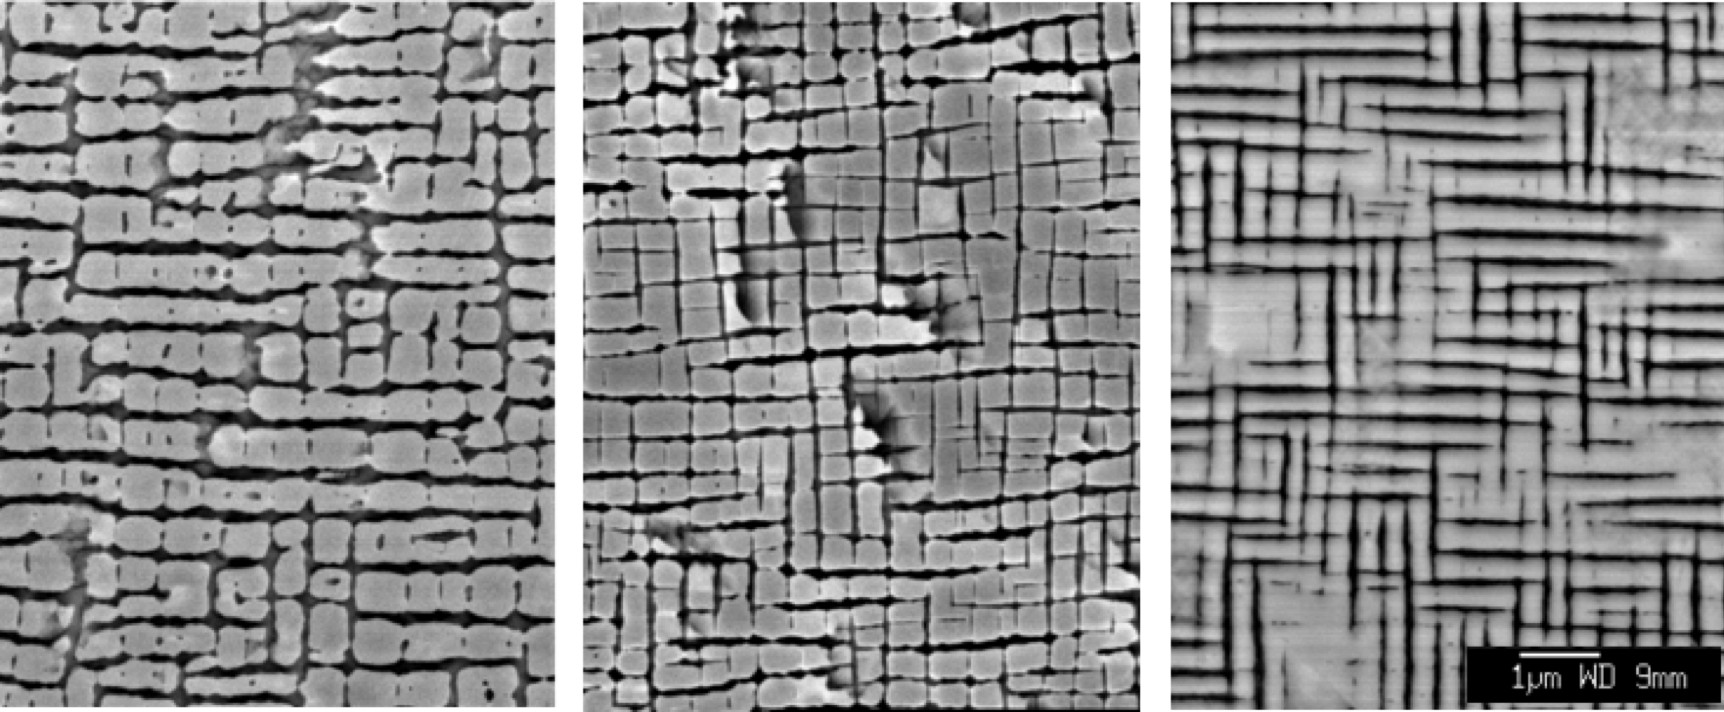
\includegraphics{LDSXInterrupted_50}
\caption{LDSX--1, 6 and 8: as interrupted crept + 50 hours at 950\celsius}\label{fig:LDSXInterrupted_50}
\end{center}
\end{figure} 
%
\begin{figure}[hp]
\begin{center}
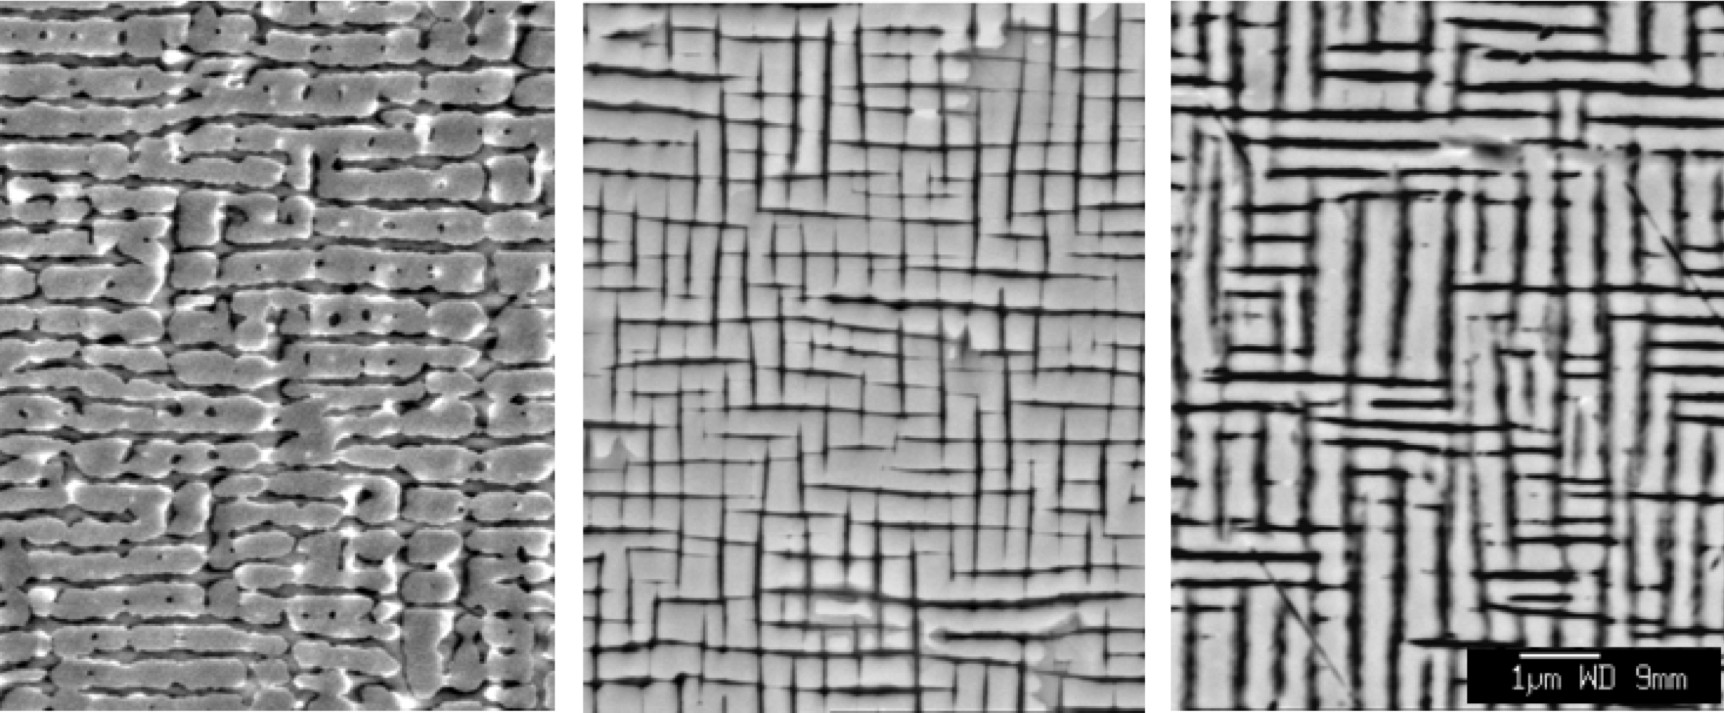
\includegraphics{LDSXInterrupted_200}
\caption{LDSX--1, 6 and 8: as interrupted crept + 200 hours at 950\celsius. }\label{fig:LDSXInterrupted_200}
\end{center}
\end{figure} 
%
\begin{figure}[hp]
\begin{center}
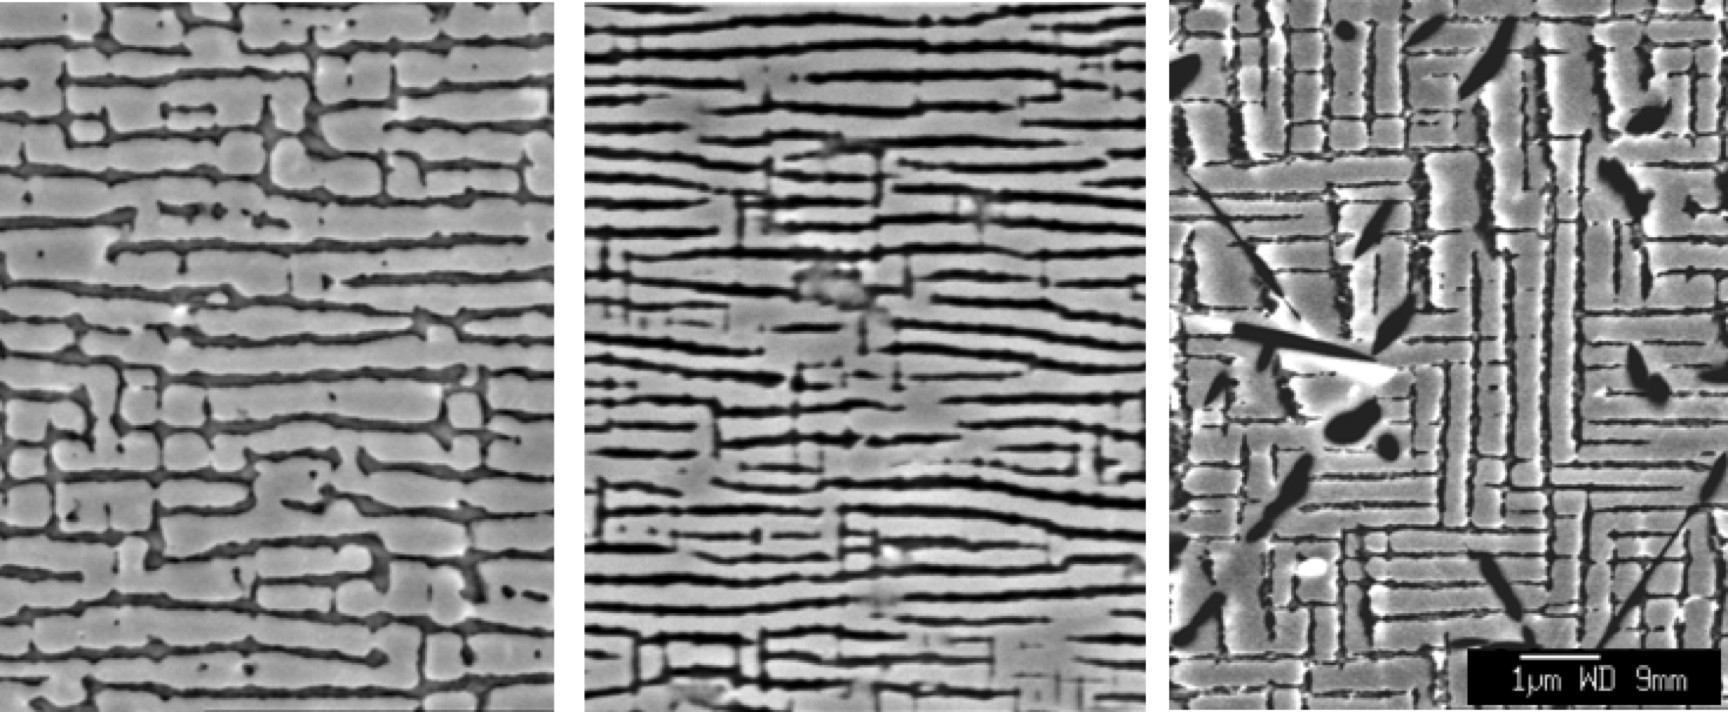
\includegraphics{LDSXInterrupted_500}
\caption{LDSX--1, 6 and 8: as interrupted crept + 500 hours at 950\celsius.}\label{fig:LDSXInterrupted_500}
\end{center}
\end{figure}
%
In LDSX--6, some TCP precipitation was seen in the dendrite core regions after 200 additional hours at 950\celsius\ (Figure \ref{fig:LDSXInterrupted_200}).  The volume fraction of precipitates is not substantial enough to adversely affect creep properties.  This is consistent with LDSX--6 having the longest creep life.  

Dislocations were observed in the $\gamma$ channels of the as heat treated LDSX--8 in TEM (Figure \ref{fig:LDSX8disloc}).  They were unobservable in the as heat treated SEM sample (Figure \ref{fig:LDSXAsAged}) because the specimen was sectioned at an angle to the $\{001\}$ plane, which did not allow large portions of $\gamma$ channels to be observed.  The presence of dislocations prior to application of stress is quite unusual.  Dislocation networks became noticeable in the dendritic regions of the interrupted creep specimen after a subsequent thermal exposure of 10 hours (Figure \ref{fig:LDSXInterrupted_10}).  Their density increased with thermal exposure length.  Their presence indicates that the $\gamma$/$\gamma'$ interfaces have lost coherency by forming these stress-relieving networks (Figure \ref{fig:LDSX8disloc}).  

LDSX--8 is microstructurally unstable.  Rampant precipitation was observed after 200 hours at 950\celsius, and most dendritic regions contained substantial TCP precipitates (Figure \ref{fig:LDSXInterrupted_200}).  This extensive TCP precipitation is detrimental to creep properties, as it depletes the surrounding microstructure of strengthening elements.  The removal of these elements reduces the alloy's lattice misfit, but rafting was not halted nor reversed, as can be seen in the specimen that had been exposed for 500 hours at 950\celsius\ (Figure \ref{fig:LDSXInterrupted_500}). 

It is difficult to isolate the influence that lattice misfit has on creep from the influence of the extent of TCP precipitatation; these two factors have a very strong correlation, as can be seen in LDSX--8.  Lattice misfit becomes more negative upon the addition of select refractory elements; this also increases rafting and promotes TCP precipitation. 

The premature failure of LDSX--8 in creep will have to be attributed to both its highly rafted labyrinth structure and the extensive precipitation of TCPs.  Figure \ref{fig:LDSXCreep} shows time to \% strain for the three alloys.  LDSX--8 showed the poorest properties and took 60 hours to reach 1\% elongation.  The specimen with the closest thermal history available had been interrupted after 2 hours of primary creep at 950\celsius, and subjected to a further 50-hour thermal exposure (Figure \ref{fig:LDSXInterrupted_50}).  This specimen has a large population of dislocation networks.  The TCP precipitates visible are sparsely scattered, and are unlikely to adversely affect the mechanical properties of the alloy substantially.  From this, it can be said that the poorer performance of LDSX--8, as seen from its shorter time to 1\% elongation at 950\celsius\ when compared to LDSX--6, is exclusively due to its labyrinth structure.  The creep rupture time for LDSX--8 is even worse; it is half that of LDSX--6.  At this stage, TCP precipitation probably has a stronger negative influence than the labyrinth structure.

MacKay and Ebert state that the wider $\gamma$ channels resulting from rafting would adversely affect creep-rates at 950\celsius.  Comparing the times to 0.5\% strain of the three alloys, strain rates increase with increasing misfit.  The alloy with the least propensity to raft, LDSX--1, has the longest time to 1\% strain.  This is consistent with the opinion of MacKay and Ebert ~\cite{mackay83}.  When we look at the times to 2\% strain, the strain rate of LDSX--6 between 0.5\% and 2\% is markedly slower than LDSX--1, as the time to 2\% strain is equal in both alloys.  These results suggest that wider $\gamma$ channels impact creep only to a small extent, and this impact is limited to initial creep strain.  These channels may allow the dislocations to travel a larger distance with ease, but once the dislocations encounter a $\gamma'$ precipitate, they are captured at the $\gamma$/$\gamma'$ interface, and cannot travel further.  In fact, we suggest that the $\gamma'$ precipitates in LDSX--6 may be stronger than those in LDSX--1 due to the higher content of refractory elements present, and they pose a larger resistance to precipitate cutting by dislocations, thereby improving creep resistance and allowing for LDSX--6 to display a longer time to creep rupture than LDSX--1.

An increase of misfit improves creep performance, but a misfit larger than the optimum level is is detrimental to creep.  We do not see an adverse effect due to the extent of rafting; LDSX--6 rafts to a greater extent than LDSX--1, but has better creep properties.  A negative effect is only seen when the labyrinth structure is present. 

The diffusion coefficient of $\gamma$ is one magnitude higher than that of $\gamma'$, and allows the refractory elements to cluster together with more ease in the former, nucleating TCP precipitates ~\cite{reed06}.  This is why TCP precipitates are mostly located in the wider $\gamma$ channels where there are substantial dislocation networks.  These networks serve as fast diffusion paths for the slow-diffusing refractory atoms to agglomerate into TCP precipitates.  It is interesting to note that although LDSX--6 is less stable than LDSX--1 with respect to TCP precipitation, it is also stronger with the slowest creep at all strains above 2\% (Figure \ref{fig:LDSXCreep}).   

These results suggest there is an upper limit on the useful magnitude of the negative misfit and thus the concentration of refractory elements used to strengthen the $\gamma$-matrix at intermediate temperatures.  At lower temperatures, misfit appears beneficial for creep at 750\celsius.  But as the temperature rises, high misfit can cause spontaneous rafting to give a labyrinth structure.  This appears to be detrimental for creep at 950\celsius\ even before substantial TCP precipitation is observed.  This can be tested by producing a microstructure in LDSX--8 without the labyrinth rafting through a suitable heat treatment.
%
\begin{figure}[H]
\begin{center}
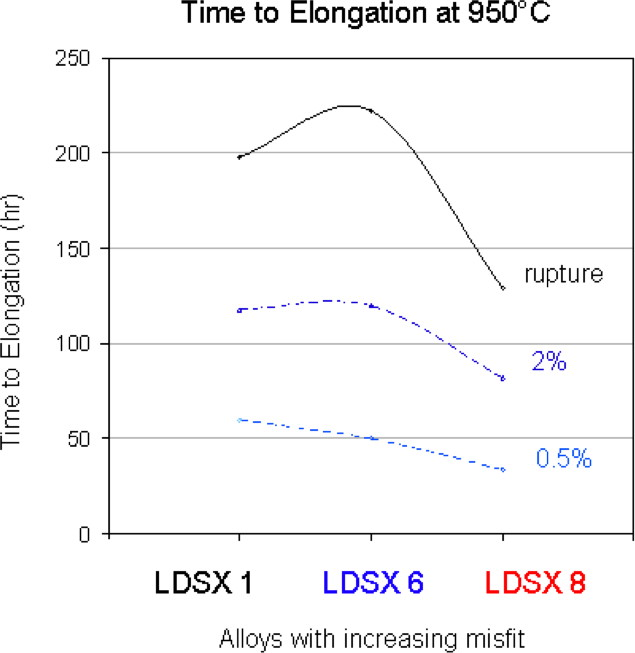
\includegraphics[width=9cm]{LDSXCreep}
\caption{Time to \% percent elongation of LDSX--1, 6 and 8 at 950\celsius/ 375\mega\pascal.}
\label{fig:LDSXCreep}
\end{center}
\end{figure}
%
\begin{figure}[H]
\begin{center}
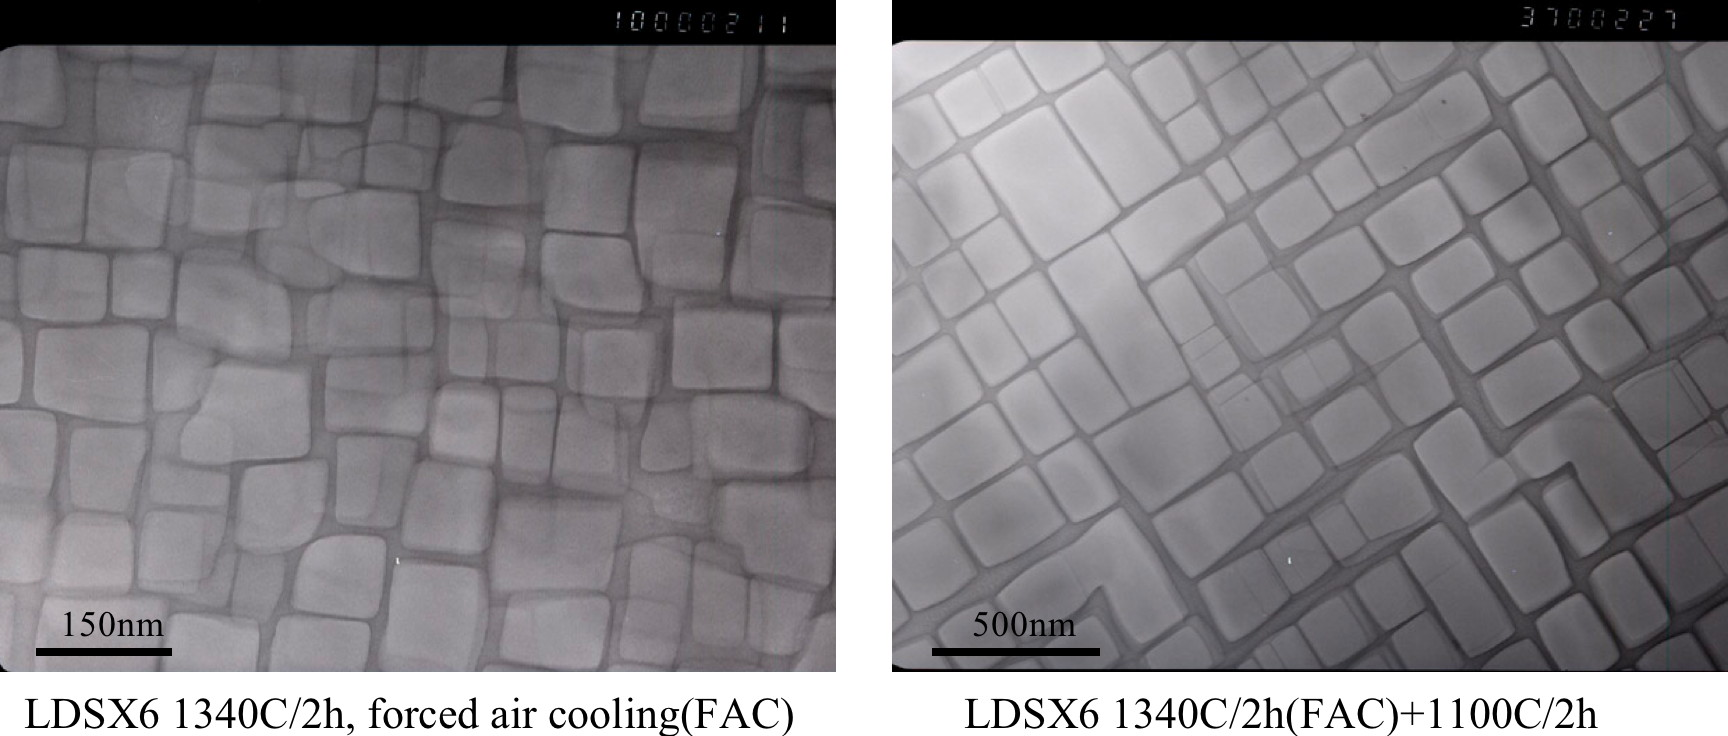
\includegraphics{LDSX6HT}
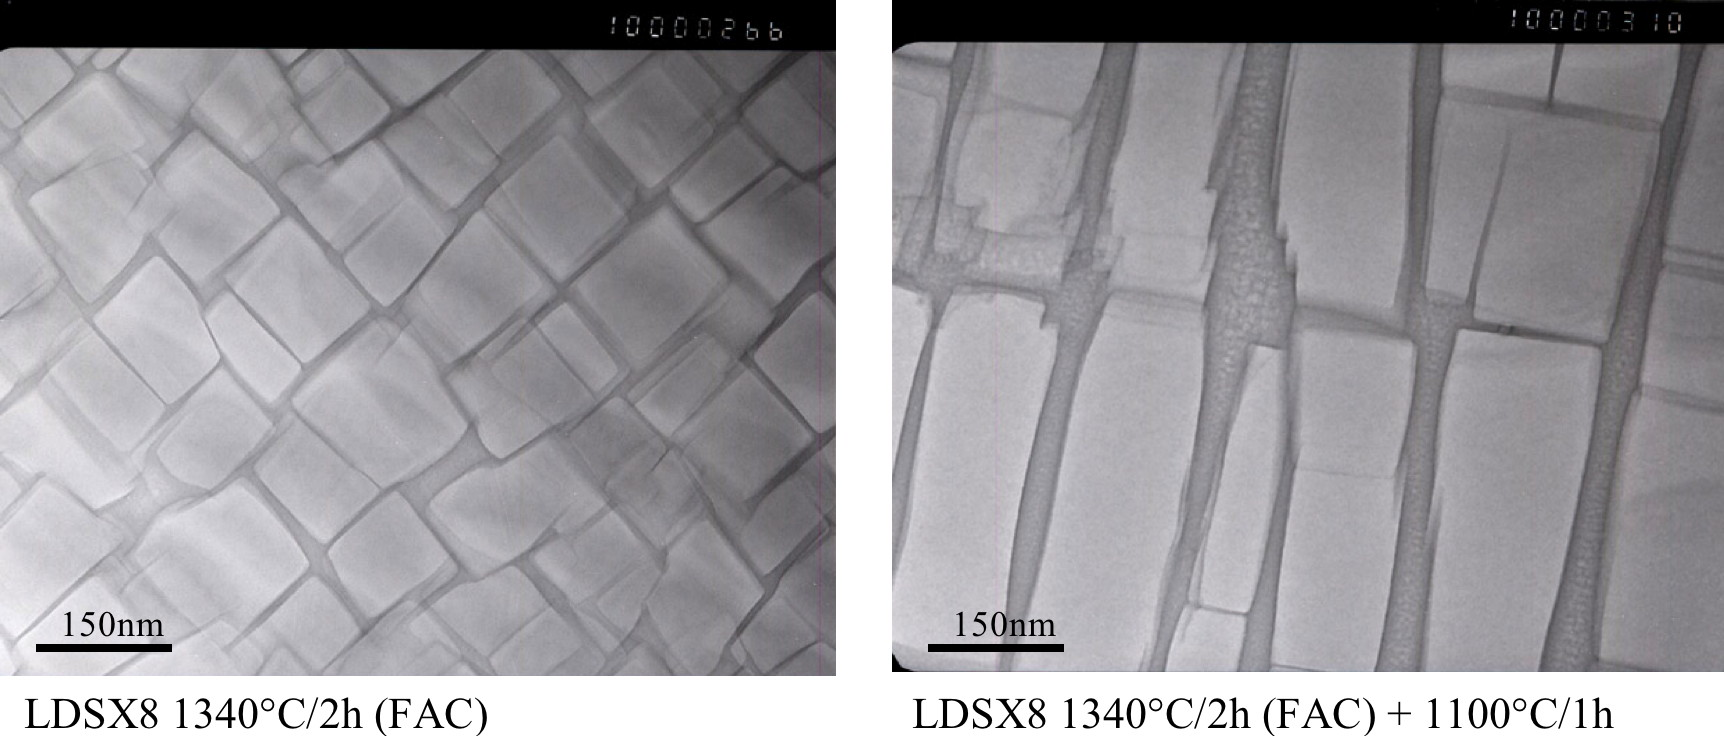
\includegraphics{LDSX8HT}
\caption{TEM micrographs of LDSX--6 and 8 after various heat treatments.}
\label{fig:LDSXHT}
\end{center}
\end{figure}
\vspace{-8mm}
%
Typically, a nickel-base superalloy that has been homogenised has to undergo an ageing treatment to achieve a uniform distribution of cubiodal $\gamma'$ precipitates.  This ageing treatment is performed at 1100\celsius\ for a few hours, as this is the temperature required for the diffusion step of the application of low-cost platinum-aluminised bond coats used as protection against high-temperature corrosion and oxidation ~\cite{reed06}.  As seen in Figure \ref{fig:LDSXHT}, the $\gamma'$ precipitates of LDSX--6, become more cuboidal and orderly after 2 hours at 1100\celsius .  

Figure \ref{fig:LDSXHT} shows the microstructures of LDSX--6 and 8 after an additional solution heat treat of 2 hours at 1340\celsius\ followed by an air quench.  This process produces a finer $\gamma'$ size than conventional cool in a commercial furnace.  In the case of the highly misfitting LDSX--8, precipitate coalescence occurs after 1 hour at 1100\celsius, which is disadvantageous for low and intermediate temperature creep.  The as-homogenised LDSX--8 specimen that underwent an additional 1340\celsius\ for 2 hours seems to have a sufficiently optimised microstructure; the $\gamma'$ precipitates are cubiodal.  If the labyrinth structure seen in the as-aged specimen is detrimental to the creep properties of LDSX--8, the as-homogenised specimen should out-perform the as-aged specimen in creep.  A creep test at 950\celsius/ 375\mega\pascal\ will be conducted on this as-homogenised sample and compared to the creep results of the as-aged specimen.  This will indicate the extent of which labyrinth rafting is causing the poor creep properties.

\subsection{Measurement of Lattice Misfit}

Two-dimensional and three-dimensional plots (Figure \ref{fig:3Dplot}) of intensity in reciprocal space were obtained at the ESRF. 





There are two $\gamma$ peaks due to the different lattice parameters of the constrained $\gamma$ in the vertical channels and the unconstrained $\gamma$ in the horizontal channels.  The peaks from $\gamma'$ and the constrained $\gamma$ were fitted, and theirlattice parameters were used to calculate the lattice misfits using Equation \eqref{eq:misfit}.  The calculated misfit values (Table \ref{tab:misfitesrf}) are higher than the predicted values (Table \ref{tab:misfitjmatpro}). 
 
\begin{figure}[H]
\begin{center}
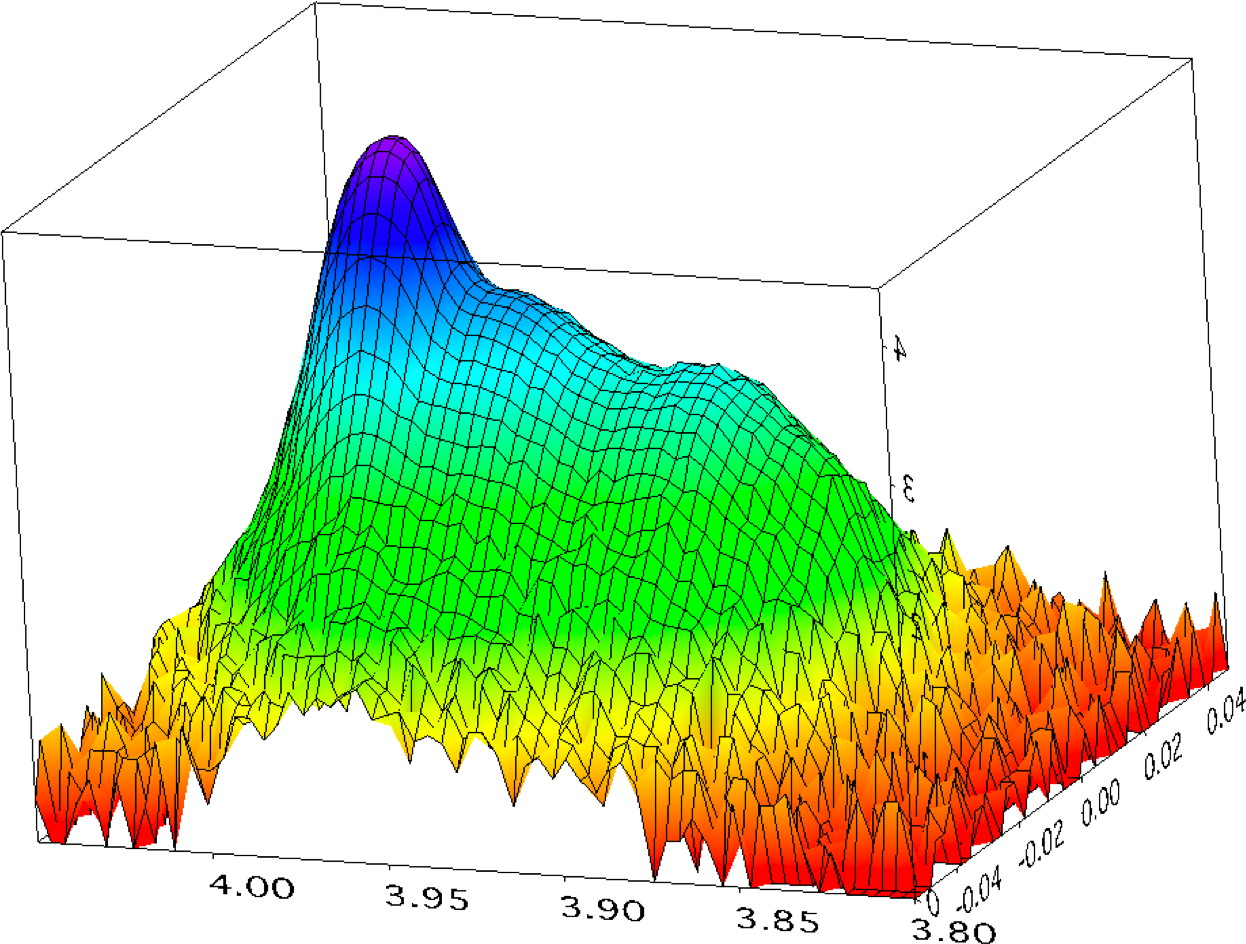
\includegraphics{3Dplot}
\caption{3D plot of LDSX--8 as HT}\label{fig:3Dplot}
\end{center}
\end{figure}

 
%
\begin{table}[H]
\begin{center}
\begin{tabular}{l c c c c} 
\hline
\hline
Alloy & 	Phase    &	Reciprocal lattice distance   &Lattice distance &	Misfit 	\\
\hline
\multirow{2}{*}{LDSX--1}&	$\gamma$ &	3.96944					&3.62029	&	\multirow{2}{*}	{-0.77\%}	\\
	 &	$\gamma'$&	4.00004					&3.59259	&				\\
\multirow{2}{*}{LDSX--6}&	$\gamma$ &	3.96443					&3.62486	&	\multirow{2}{*}	{-0.85\%}	\\
 	 &	$\gamma'$&	3.99827					&3.59418	&				\\
\multirow{2}{*}{LDSX--8}&	$\gamma$ &	3.96783					&3.62176	&	\multirow{2}{*}	{-0.78\%}	\\
	 &	$\gamma'$&	3.99896					&3.59356	&				\\
\hline
\hline
\end{tabular}
\end{center}
\caption{Lattice misfit values of LDSX--1, 6 and 8, obtained at the ESRF. }
\label{tab:misfitesrf}
\end{table}


\begin{table}[H]
\begin{center}
\begin{tabular}{l c c } 
\hline
\hline
Alloy&	Temp (\celsius) &	Misfit (\%)\\
\hline
&	25	&-0.11\\
CMSX-4	&900	&-0.25\\
	&1100&-0.25\\
	\hline
&	25	&-0.22\\
LDSX--1	&900	&-0.30\\
	&1100&	-0.30\\
	\hline
&	25	&-0.31\\
LDSX--2	&900	&-0.41\\
	&1100&	-0.41\\
	\hline
&	25&	-0.36\\
LDSX--3	&900&	-0.47\\
	&1100&	-0.44\\
	\hline
&	25	&-0.22\\
LDSX--4	&900	&-0.30\\
	&1100&	-0.30\\\hline
&	25&	-0.25\\
LDSX--5	&900	&-0.33\\
	&1100&	-0.33\\
	\hline
&	25&	-0.28\\
LDSX--6	&900	&-0.36\\
	&1100&	-0.35\\
	\hline
&	25&	-0.39\\
LDSX--7	&900	&-0.44\\
	&1100&	-0.44\\
	\hline
&	25&	-0.39\\
LDSX--8	&	900&	-0.47\\
	&	1100&	-0.49\\
\hline
\hline
\end{tabular}
\end{center}
\caption{Lattice misfit values of LDSX--1, 6 and 8, predicted by JMatPro$^{\copyright}$. }
\label{tab:misfitjmatpro}
\end{table}


\section{Summary/Conclusion}
Materials that have operating capabilities at higher temperatures are required for fuel efficiency.  The microstructural stability of three of the most advanced 4$^{th}$ generation alloys, LDSX--1, 6, and 8, with representative low, medium and high misfit, was evaluated. Misfit values of the alloys were measured using X-ray diffraction at a synchrotron.  Interrupted creep specimens were subjected to thermal exposure at 950\celsius, the temperature that the specimens were crept at, for a further 10, 50, 100, 200, 500 or 3000 hours.  The more heavily alloyed LDSX 6 with higher lattice misfit took a longer time than LDSX 1 to reach the same elongation.  The most heavily alloyed LDSX 8, suffered from premature rupture, and had half the rupture life of LDSX 1. 

Dislocations were observed in the $\gamma$ channels of the as heat treated LDSX 8 in TEM.  The presence of dislocations prior to application of stress is quite unusual.  Dislocation networks became noticeable in the dendritic regions of the interrupted creep specimen after a subsequent thermal exposure of 10 hours.  Their density increased with thermal exposure length.  Their presence indicates that the $\gamma$/$\gamma'$ interfaces have lost coherency by forming these stress-relieving networks. LDSX 8 is microstructurally unstable. Rampant precipitation was observed after 200 hours at 950\celsius, and most dendritic regions contained substantial TCP precipitates.  This extensive TCP precipitation is detrimental to creep properties, as it depletes the surrounding microstructure of strengthening elements.  The removal of these elements reduced the alloy's lattice misfit, but rafting was not halted nor reversed, as can be seen in the specimen that had been exposed for 500 hours at 950\celsius. 

It is difficult to isolate the influence that lattice misfit has on creep from the influence of the extent of TCP precipitatation; these two factors have a very strong correlation, as can be seen in LDSX 8. Lattice misfit becomes more negative upon the addition of select refractory elements; this also increases rafting and promoted TCP precipitation.  The premature failure of LDSX 8 in creep has been attributed to both its highly rafted labyrinth structure and the extensive precipitation of TCPs.  At 1\% elongation, the poorer performance of LDSX 8, as seen from its shorter time to 1\% elongation at 950\celsius\ when compared to LDSX 6, was exclusively due to its labyrinth structure.  The creep rupture time for LDSX 8 was even worse; it was half that of LDSX 6.  At this stage, TCP precipitation probably had a stronger negative influence than the labyrinth structure.

These results suggested that wider $\gamma$ channels impact creep only to a small extent, and this impact is limited to initial creep strain.  These channels may allow the dislocations to travel a larger distance with ease, but once the dislocations encounter a $\gamma'$ precipitate, they are captured at the $\gamma$/$\gamma'$ interface, and cannot travel further.  In fact, we suggest that the $\gamma'$ precipitates in LDSX 6 may be stronger than those in LDSX 1 due to the higher content of refractory elements present.  They posed a larger resistance to precipitate cutting by dislocations, thereby improved creep resistance and allowed for LDSX 6 to display a longer time to creep rupture than LDSX 1.

An increase of misfit improved creep performance, but a misfit larger than the optimum level is detrimental to creep.  We do not see an adverse effect due to the extent of rafting; LDSX 6 rafted to a greater extent than LDSX 1, but had better creep properties.  A negative effect is only seen when the labyrinth structure is present.

Measurements of the lattice parameters of the gamma matrix phases and $\gamma'$ precipitate phases of the alloys were performed on the BM28 beamline at the European Synchrotron Radiation Facility (ESRF) in Grenoble, France.  The measured misfit values were higher than the values predicted by JMatPro$^{\copyright}$ as can be seen in Tables \ref{tab:misfitsref} and \ref{tab:misfitjmatpro}.

These results suggest there is an upper limit on the useful magnitude of the negative misfit and thus the concentration of refractory elements used to strengthen the $\gamma$-matrix at intermediate temperatures.  At lower temperatures, misfit appeared beneficial for creep at 750\celsius. But at higher temperatures, high misfit caused spontaneous rafting and gave a labyrinth structure.  This appeared to be detrimental for creep at 950\celsius\ even before substantial TCP precipitation is observed.  This will be confirmed by producing a microstructure in LDSX 8 without the labyrinth rafting through a suitable heat treatment.

